% !TEX program = lualatex
\documentclass[12pt,a4paper]{article}

% Sprache: deutsche Silbentrennung, »Inhaltsverzeichnis«, »Abbildung«
\usepackage{polyglossia}
\setdefaultlanguage{german}

% Schrift für Text und Formeln
\usepackage{fontspec}
\usepackage{unicode-math}
\setmainfont{TeX Gyre Termes}
\setmathfont{TeX Gyre Termes Math}

% Seitenränder, Zeilenabstand, Absätze
\usepackage[left=30mm, right=25mm, top=25mm, bottom=25mm]{geometry}
\usepackage{setspace}
\onehalfspacing
\setlength{\parindent}{0pt}
\setlength{\parskip}{6pt}

% Tabellen, Einheiten, Bilder, Diagramme
\usepackage{booktabs}
\usepackage[locale=DE]{siunitx}
\usepackage{graphicx}
\usepackage{float}
\usepackage{tikz}

% Quellen
\usepackage[style=authoryear, backend=biber]{biblatex}
\addbibresource{literatur.bib}

% Klickbare Verweise im PDF
\usepackage[hidelinks]{hyperref}

\begin{document}

% ------------------------------------------------------------ Titelseite
\begin{titlepage}
  \centering
  \vspace*{30mm}
  {\Large Facharbeit im Fach Physik\par}
  \vspace{15mm}
  {\huge\bfseries Wie lange schwingt ein Pendel?\par}
  \vspace{6mm}
  {\Large Die Schwingungsdauer eines Fadenpendels\\ im Versuch und in der Theorie\par}
  \vfill
  {\large Alex Schmidt\par}
  \vspace{3mm}
  {\large Kurs Physik 11 · Schuljahr 2026/27\par}
  \vspace{3mm}
  {\large Abgabe: 15. Oktober 2026\par}
\end{titlepage}

\tableofcontents
\newpage

% ------------------------------------------------------------ Text
\section{Einleitung}

Eine Kugel an einem Faden schwingt hin und her. Ein solches \emph{Fadenpendel}
war jahrhundertelang das Herz jeder genauen Uhr. In dieser Arbeit untersuche
ich, wovon es abhängt, wie lange eine Schwingung dauert: von der Länge des
Fadens, von der Masse der Kugel oder davon, wie weit man sie auslenkt.

\section{Theorie}

Für kleine Auslenkungen hängt die Schwingungsdauer~$T$ nur von der Länge~$l$
des Fadens und der Fallbeschleunigung~$g$ ab \parencite{tipler2019}:
\begin{equation}
  T = 2\pi \sqrt{\frac{l}{g}}
  \label{eq:schwingungsdauer}
\end{equation}
Die Masse der Kugel kommt in Gleichung~\eqref{eq:schwingungsdauer} nicht vor.
Für größere Auslenkungen wird $T$ etwas länger.\footnote{Bei einer Auslenkung
von \ang{20} ist der Unterschied kleiner als ein Prozent \parencite{pendel}.}

\section{Versuch}

\subsection{Aufbau}

An einem Stativ hängt eine Stahlkugel an einem dünnen Faden
(Abbildung~\ref{fig:aufbau}). Die Länge des Fadens lässt sich verstellen.

\begin{figure}[H]
  \centering
  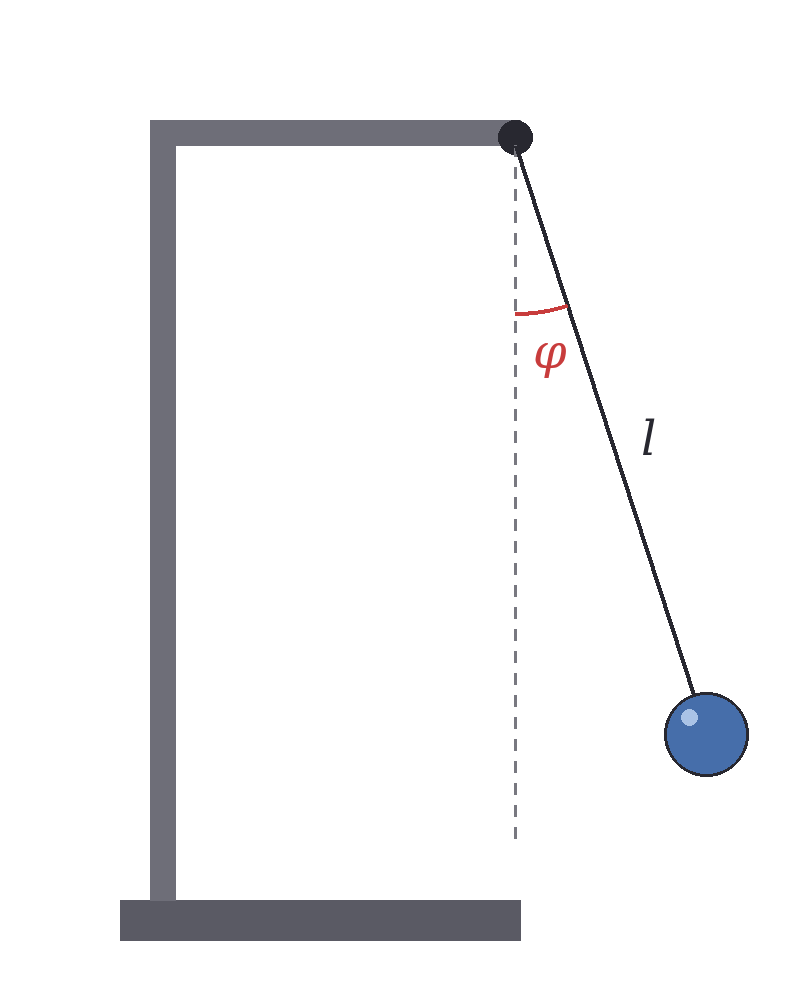
\includegraphics[width=0.45\textwidth]{aufbau.png}
  \caption{Aufbau des Versuchs: ein Fadenpendel an einem Stativ}
  \label{fig:aufbau}
\end{figure}

\subsection{Durchführung}

\begin{enumerate}
  \item Die Fadenlänge~$l$ einstellen und messen.
  \item Die Kugel um etwa \ang{10} auslenken und loslassen.
  \item Die Zeit für zehn Schwingungen stoppen und durch zehn teilen.
\end{enumerate}

\subsection{Messwerte}

\begin{table}[H]
  \centering
  \caption{Gemessene Schwingungsdauer für verschiedene Fadenlängen}
  \label{tab:messwerte}
  \begin{tabular}{ccc}
    \toprule
    Länge $l$ in \unit{\metre} & 10 Schwingungen in \unit{\second} & $T$ in \unit{\second} \\
    \midrule
    0,20 &  9,0 & 0,90 \\
    0,40 & 12,7 & 1,27 \\
    0,60 & 15,6 & 1,56 \\
    0,80 & 17,9 & 1,79 \\
    1,00 & 20,1 & 2,01 \\
    \bottomrule
  \end{tabular}
\end{table}

\section{Auswertung}

Abbildung~\ref{fig:diagramm} zeigt die Messwerte aus Tabelle~\ref{tab:messwerte}
zusammen mit der Kurve aus Gleichung~\eqref{eq:schwingungsdauer} für
$g = \qty{9,81}{\metre\per\second\squared}$.

\begin{figure}[H]
  \centering
  \begin{tikzpicture}[x=10cm, y=2.5cm]
    % Achsen mit Beschriftung
    \draw[->] (0,0) -- (1.1,0) node[right] {$l$ in \unit{\metre}};
    \draw[->] (0,0) -- (0,2.3) node[above] {$T$ in \unit{\second}};
    \foreach \x in {0.2, 0.4, 0.6, 0.8, 1.0}
      \draw (\x,0.03) -- (\x,-0.03) node[below] {\num{\x}};
    \foreach \y in {0.5, 1.0, 1.5, 2.0}
      \draw (0.01,\y) -- (-0.01,\y) node[left] {\num{\y}};
    % Theorie: T = 2 pi sqrt(l / g)
    \draw[thick, blue, domain=0:1.05, samples=60]
      plot (\x, {2*pi*sqrt(\x/9.81)});
    % Messwerte
    \foreach \l/\t in {0.2/0.90, 0.4/1.27, 0.6/1.56, 0.8/1.79, 1.0/2.01}
      \fill[red] (\l,\t) circle (2.5pt);
  \end{tikzpicture}
  \caption{Messwerte (rot) und die Kurve aus der Theorie (blau)}
  \label{fig:diagramm}
\end{figure}

Die Messwerte liegen sehr nah an der Kurve. Stellt man
Gleichung~\eqref{eq:schwingungsdauer} nach $g$ um, ergibt sich aus der Messung
mit $l = \qty{1,00}{\metre}$ der Wert $g = \frac{4\pi^2 l}{T^2}
\approx \qty{9,77}{\metre\per\second\squared}$.

\section{Fazit}

Die Schwingungsdauer eines Fadenpendels hängt von der Länge des Fadens ab,
nicht aber von der Masse der Kugel. Vervierfacht man die Länge, verdoppelt
sich die Schwingungsdauer. Die Messungen bestätigen die Theorie.

\printbibliography

\newpage
\section*{Selbstständigkeitserklärung}

Ich erkläre, dass ich diese Facharbeit selbstständig angefertigt und nur die
angegebenen Quellen und Hilfsmittel verwendet habe.

\vspace{20mm}
\rule{60mm}{0.4pt}\\
Ort, Datum, Unterschrift

\end{document}
